\section{tasks::scattering Class Reference}
\label{classtasks_1_1scattering}\index{tasks::scattering@{tasks::scattering}}
Inheritance diagram for tasks::scattering::\begin{figure}[H]
\begin{center}
\leavevmode
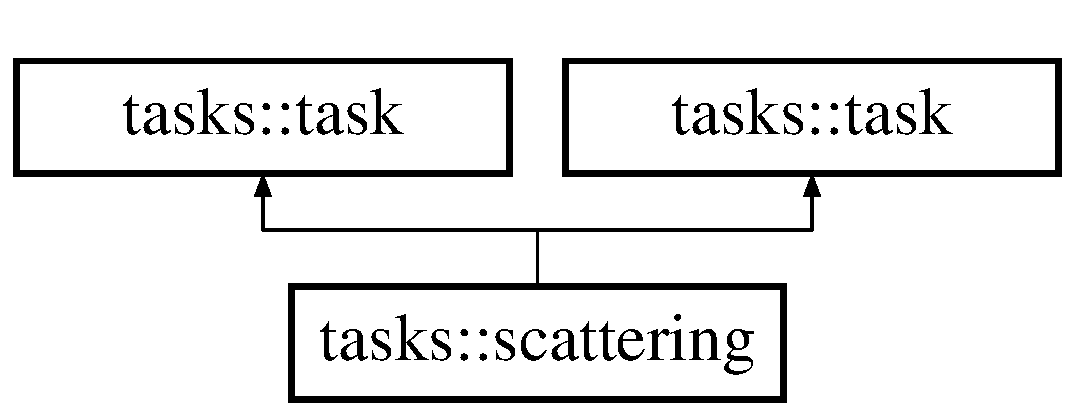
\includegraphics[height=2cm]{classtasks_1_1scattering}
\end{center}
\end{figure}
\subsection*{Public Member Functions}
\begin{CompactItemize}
\item 
def \textbf{run}\label{classtasks_1_1scattering_6a8bc937f9d90d5b323c43181cb49c90}

\item 
def \textbf{run}\label{classtasks_1_1scattering_6a8bc937f9d90d5b323c43181cb49c90}

\end{CompactItemize}
\subsection*{Static Public Attributes}
\begin{CompactItemize}
\item 
string \textbf{name} = '{\bfscattering}'\label{classtasks_1_1scattering_97d7e7a54a8fa2fb744b92b4d2f6b264}

\item 
string \textbf{button\-Text} = 'Subtract {\bfscattering}'\label{classtasks_1_1scattering_10415ad70b14c3799a96c2a8e04e4424}

\item 
string \textbf{suffix} = 'scat'\label{classtasks_1_1scattering_de1786871cb2f4d87faa22845f407226}

\item 
list \textbf{prereq} = ['{\bfpreproc}']\label{classtasks_1_1scattering_5d6fbe8a4bf1272f8da527289b3babaf}

\end{CompactItemize}


\subsection{Detailed Description}


\footnotesize\begin{verbatim}Model and subtract the scattered light in an image. The level of scattered
   light is estimated from the level between the individual orders.
\end{verbatim}
\normalsize
 



The documentation for this class was generated from the following files:\begin{CompactItemize}
\item 
old/PANICtool-1.0/tasks.py\item 
old/tasks.py\end{CompactItemize}
